\documentclass[12pt]{article}
\usepackage{geometry}                % See geometry.pdf to learn the layout options. There are lots.
\geometry{letterpaper}                   % ... or a4paper or a5paper or ... 
%\geometry{landscape}                % Activate for for rotated page geometry
\usepackage[parfill]{parskip}    % Activate to begin paragraphs with an empty line rather than an indent
\usepackage{daves,fancyhdr,natbib,graphicx,dcolumn,amsmath,lastpage,url}
\usepackage{amsmath,amssymb,epstopdf,longtable}
\usepackage{paralist}  % need to properly formulate standard answer blocks
\usepackage[final]{pdfpages}
\DeclareGraphicsRule{.tif}{png}{.png}{`convert #1 `dirname #1`/`basename #1 .tif`.png}
\pagestyle{fancy}
\lhead{CE 3305 Fluid Mechanics; Exercise Set 13}
\rhead{Name:\_\_\_\_\_\_\_\_\_\_\_\_\_\_\_\_\_\_\_\_\_\_\_\_\_\_\_\_\_\_\_\_\_\_}
\lfoot{REVISION A}
\cfoot{}
\rfoot{Page \thepage\ of \pageref{LastPage}}
\renewcommand\headrulewidth{0pt}
%%%%%%%%%%%%%%%%%%%%%%%%%%%%%%%%%%%%
\begin{document}
%%%%%%%%%%%%%%%%%%%%%%%%%%%%%%%%%%%
\begingroup
\begin{center}
{\textbf{{ CE 3305 Engineering Fluid Mechanics} \\ Exercise Set 13 \\ Summer 2018 -- GERMANY} }
\end{center}
\endgroup
\begingroup
~\newline
\textbf{Purpose} :  Conservation of mass and energy\\
\textbf{Assessment Criteria} : Completion, plausible solutions, use \textbf{R} as a calculator. \\~\\
\textbf{Exercises}

\begin{enumerate}
\item (Problem 5.74 pg 202)  Figure \ref{fig:GasSparger} is a schematic of a pipe with a series of holes used to sparge (introduce gas bubbles) gas into a larger volume.  
The volumetric flow rate through each hole depends on the pressure difference across the hole and is given by \\
\begin{equation}
Q = 0.67 A_0 (\frac{2 \Delta p }{\rho})^{\frac{1}{2}}
\end{equation}
where $A_0$ is the area of a hole, $\Delta p$ is the pressure difference across the hole, and $\rho$ is the density of gas in the pipe.
If the pipe is sufficiently large, the pressure will be uniform along the pipe.
A distribution pipe for air at 20$^o~C$ is 0.5 meters in diameter and 10 $m$ long. 
The gage pressure in the pipe is 100 $Pa$.
The pressure outside the pipe is atmospheric at 1 $bar$.
The hole diameter is 2.5 $cm$, and there are 50 holes per meter length of pipe.
The pressure is constant in the pipe.
What is the velocity of air entering the pipe?

\begin{figure}[h!] %  figure placement: here, top, bottom, or page
   \centering
   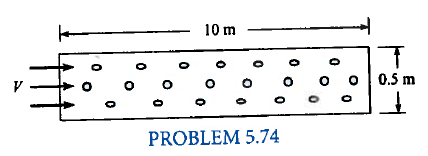
\includegraphics[width=3in]{GasSparger.jpg} 
   \caption{Gas sparger}
   \label{fig:GasSparger}
\end{figure}
\clearpage

\item (Problem 5.80 pg 203) Figure \ref{fig:Time2Drain} is a tank with a hole in the side.  Develop an apply an equation that predicts the time for the water surface in the tank to drop from $h = 3 m$ to $h = 0.5 m$.

\begin{figure}[h!] %  figure placement: here, top, bottom, or page
   \centering
   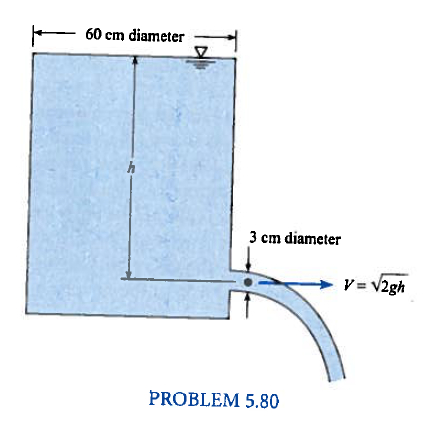
\includegraphics[width=3in]{Time2Drain.jpg} 
   \caption{Tank draining}
   \label{fig:Time2Drain}
\end{figure}

\end{enumerate}
\end{document}  